\section{Resolución por \textit{Backtracking}}
	\subsection{Descripción del algorítmo}

	La solución por Bactracking emplea recursividad en cada paso, y recorre el espacio de soluciones como si el mismo fuese un arbol en preorden.

	A continuación se propone un algoritmo para las llamadas recursivas. Para el caso inicial, se toma $Indice = 0$ y $Res = 0$.

	\begin{algorithm}[H]
		\KwData{Lista, la lista de números a pintar}

		\KwData{UltRojo, el valor del úlitmo rojo que pintamos (si existe)}

		\KwData{UltAzul, el valor del úlitmo azul que pintamos (si existe)}

		\KwData{Indice, la posición que estamos mirando ahora}

		\KwData{Res, la cantidad de elementos no pintados hasta ahora}

		\eIf{Indice == $|Lista|$}{
			Llegamos al final de la lista, no hacer nada
		}{
			Calcular el mejor resultado sin pintar

			Llamada Recursiva: \{Lista, UltRojo, UltAzul, Indice+1, Res+1\}

			Guardar ese resultado como Res

			\If{no existe UltRojo \textbf{or} UltRojo $<$ Lista[Indice]}{
				Calcular el mejor resultado pintando de Rojo

				Llamada Recursiva: \{Lista, Lista[Indice], UltAzul, Indice+1, Res\}

				Si ese resultado es menor que Res, guardarlo como Res
			}
			\If{no existe UltAzul \textbf{or} UltAzul $>$ Lista[Indice]}{
				Calcular el mejor resultado pintando de Azul

				Llamada Recursiva: \{Lista, UltRojo, Lista[Indice], Indice+1, Res\}

				Si ese resultado es menor que Res, guardarlo como Res
			}
		}

		\KwResult{Res, la menor de todas las sub-soluciones}
	\end{algorithm}

	Cabe destacar que el orden en que se calculan los posibles resultados no es relevante, en tanto se conserve el menor de todos.

	En la implementación propuesta, UltRojo y UltAzul comienzan con el menor y mayor valor representable de entero respectivamente, a modo de simplificar la comparación.

	\subsection{Cota de complejidad}

	El algoritmo propuesto realiza hasta tres llamadas recursivas en cada paso (asumiendo que el próximo número se puede pintar de cualquier color). Esto siempre es cierto para los primeros dos elementos.

	En el mejor caso, un paso cualquiera llama a solo una llamada recursiva (no se puede pintar el número).

	En cualquier llamada recursiva, el tamaño del problema a resolver disminuye en 1 (se avanza/pinta un solo número).

	La función de complejidad sería
	\[
	T(BT(n)) =
		\begin{cases}
			\text{1,} &\quad\text{si n == 0}\\
			\text{3 T(BT(n-1)) + O(1),} &\quad\text{si no} \\
		\end{cases}
	\]

	donde n es la cantidad de números restantes, es decir, $|Lista| - Indice$.

	Como, en peor caso, el algorítmo realiza 3 llamadas recursivas n veces, la complejidad resultante es \textbf{O($3^n$)}, donde n es el largo de la lista de números de entrada (es decir, cuántos numeros contiene la lista). Este es el espacio de soluciones completo, ya que cualquiera de los n elemento puede tener uno de 3 estados (existen $3^n$ combinaciones distintas).

	El caso ideal para el algoritmo es una lista de números idénticos, dando una complejidad en mejor caso de $\Omega(n^2)$, ya que solo se deben pintar 2 elementos de color distinto y hay n posiciones válidas para cada uno de ellos.

	Otro caso que vale la pena destacar es que, si la lista es estrictamente creciente/decreciente, la complejidad es de orden $\Omega(n * 2^n)$, ya que un solo elemento puede ser pintado del color opuesto, y todos los demás pueden o no ser pintados o ser pintados del color ideal (rojo si es creciente o azul en caso opuesto).

	\pagebreak
	\subsection{Gráfico de complejidad}

	El siguiente gráfico muestra la relación entre la cantidad de elementos y el tiempo que el algoritmo toma en resolver el problema. Para el mismo se utilizaron listas con contenido random, ignorando el resultado real de las mismas. A su vez, cada caso se corrió 20 veces para tratar de reducir el ruido generado por otras aplicaciones corriendo en el equipo.

	Los tiempos fueron medidos con las utilidades de \texttt{std::chrono} de C++11, corriendo dentro de los equipos de los laboratorios del DC.

	Como se puede apreciar, el tiempo crece muy rápidamente con respecto al tiempo. Originalmente las mediciones estaban en microsegundos ($seg \times 10^{-6}$), pero fueron escaladas a segundos para este caso. Casos de tamaño mayor a 50 no fueron testeados por el gran costo temporal asociado con esos tests.

	\begin{center}
	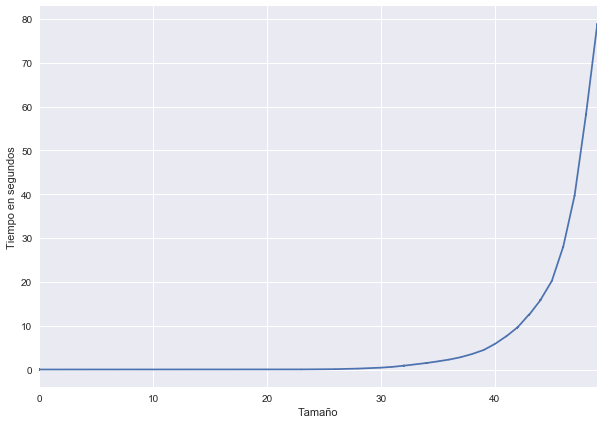
\includegraphics[width=.8\textwidth]{ej1.png}
	\end{center}